\documentclass[9pt, xcolor=table]{beamer}

\usepackage[utf8]{inputenc}
\usepackage[round, comma]{natbib}
\usepackage{amsmath}
\usepackage{hyperref}
\usepackage{amsfonts}
\usepackage{verbatim}
\DeclareMathOperator*{\argmin}{arg\,min}



\mode<presentation> {

\usetheme{Madrid}

\setbeamertemplate{navigation symbols}{} 
\useinnertheme{circles}
\definecolor{greenish}{RGB}{0, 153, 76}
\usecolortheme[named=greenish]{structure}
}

\setbeamertemplate{headline}
{%
  \begin{beamercolorbox}[ht=3.5ex,dp=1.125ex,%
      leftskip=.3cm,rightskip=.3cm plus1fil]{section in head/foot}
    \usebeamerfont{section in head/foot}\usebeamercolor[fg]{section in head/foot}%
\insertsectionnavigationhorizontal{\paperwidth}{\hskip0pt plus1fill}{\hskip0pt plus1fill}
  \end{beamercolorbox}%
  \begin{beamercolorbox}[colsep=1.5pt]{middle separation line head}
  \end{beamercolorbox}
  \begin{beamercolorbox}[colsep=1.5pt]{lower separation line head}
  \end{beamercolorbox}
}

\title[Interpretation of black box models]{Interpretation of black box models using tree-based surrogate models \newline \small{Simulations}}
\author[Sofia Loibl]{Sofia Loibl}
\institute[LMU]{LMU München}
\date{\today}

\begin{document}

\begin{frame}
\titlepage 
\end{frame}


\begin{frame}
\frametitle{Outline} 
\tableofcontents 
\end{frame}

\section{Selection Bias}
\begin{frame}{Selection Bias}
\textbf{Goal:} 

Comparison of different versions of SLIM, MOB and CTree with respect to selection bias
\vspace{0.5cm}


\textbf{Selection bias:} 

An algorithm for recursive partitionig is called unbiased when, under the conditions of the null hypothesis of independence between a response $Y$ an covariates $X_{1},...X_{m}$ the probability of selecting covariate $X_{j}$ is $1/m$ for all $j = 1,...,m$ regardless of the measurement scales of number of missing values. \citep{Hothorn.2006}
\vspace{0.5cm}

\textbf{Simulation Setting:} $1000$ simulation runs with $n= 500$
\end{frame}


\begin{frame}{Scenario Independence}
$X_{1}, X_{2} \sim U(0,1)$; 
$X_{3} \sim U(0,1)$ and rounded to one digit;
$X_{4}$ binary;
$X_{5}$ categorical with 5 levels;
$X_{6}$ categorical with 8 levels\\
$Y \sim N(0,1)$

\begin{figure}
    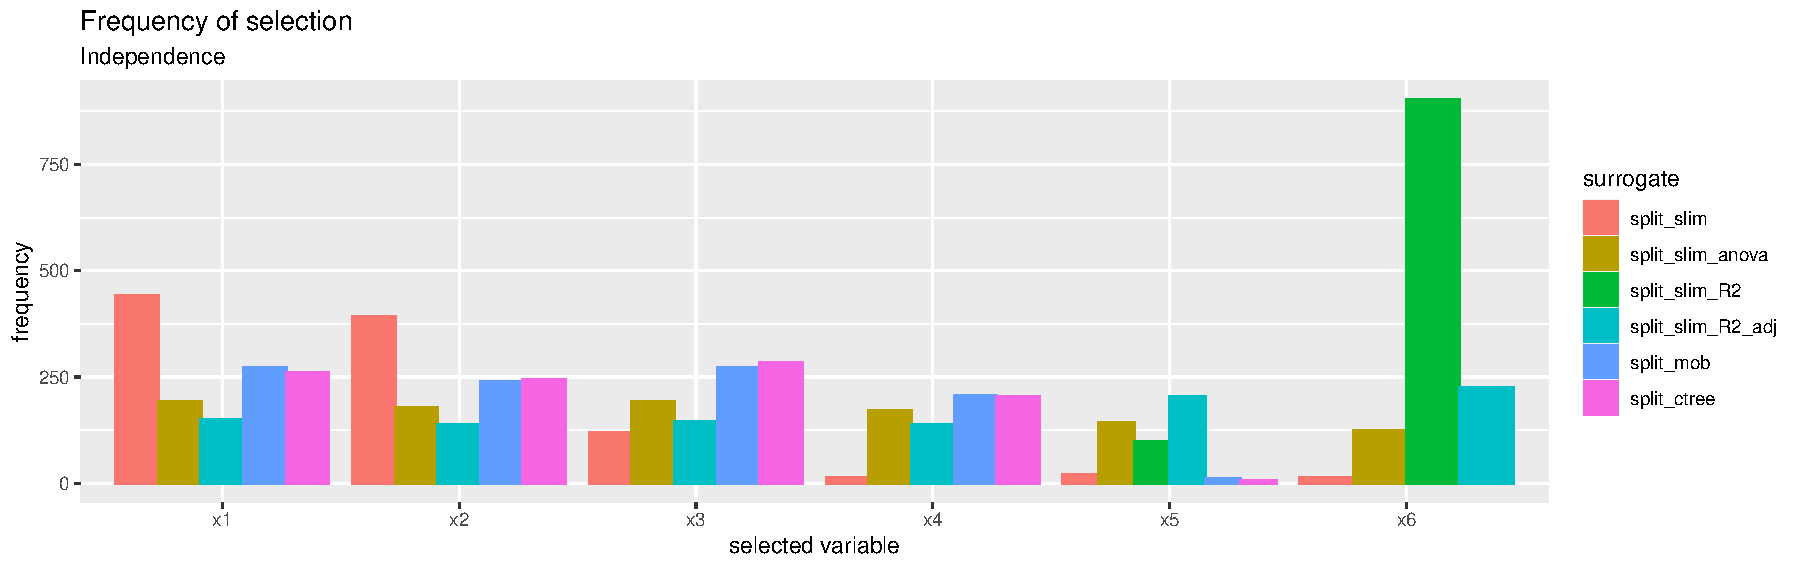
\includegraphics[width=11cm]{Figures/Selection_Bias/independence_frequency.pdf}
\end{figure}
\end{frame}


\begin{frame}{Scenario Independence small}
All $X_j \sim U(0,1)$; $X_3$ rounded to one digit, $X_4$ rounded to two digits\\
$Y \sim N(0,1)$
\begin{figure}
    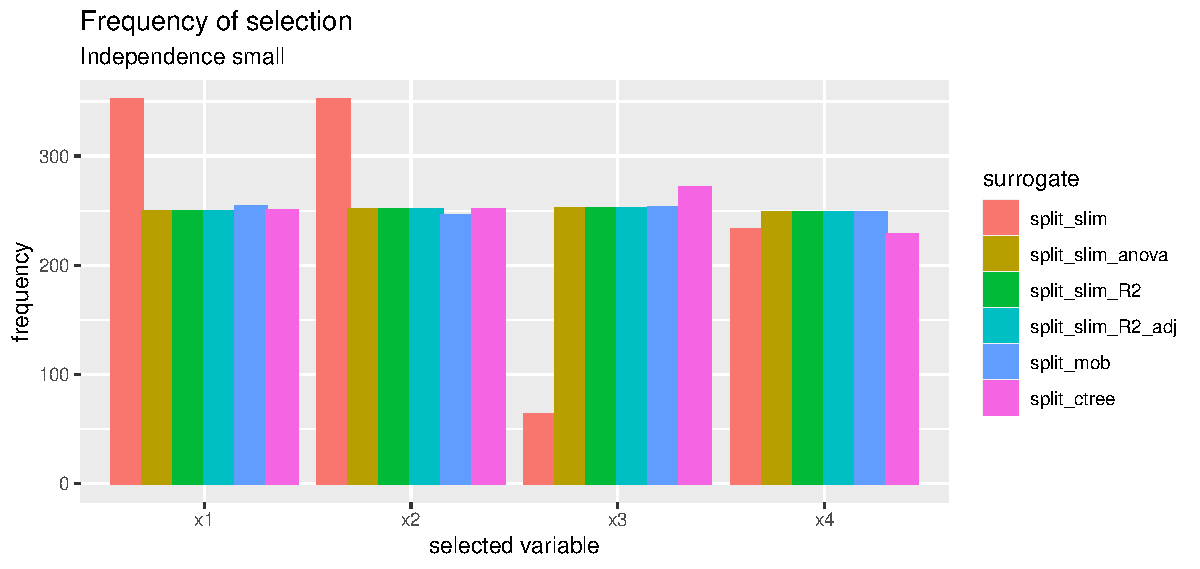
\includegraphics[width=11cm]{Figures/Selection_Bias/independence_small_frequency.pdf}
\end{figure}

\end{frame}

\begin{frame}{Scenario Interaction small}

All $X_j \sim U(0,1)$; $X_3$ rounded to one digit, $X_4$ rounded to two digits\\
$Y = X_1 + X_2 + X_3 + X_4 + X_1 X_2 + X_3 X_4 + eps$
\begin{figure}
    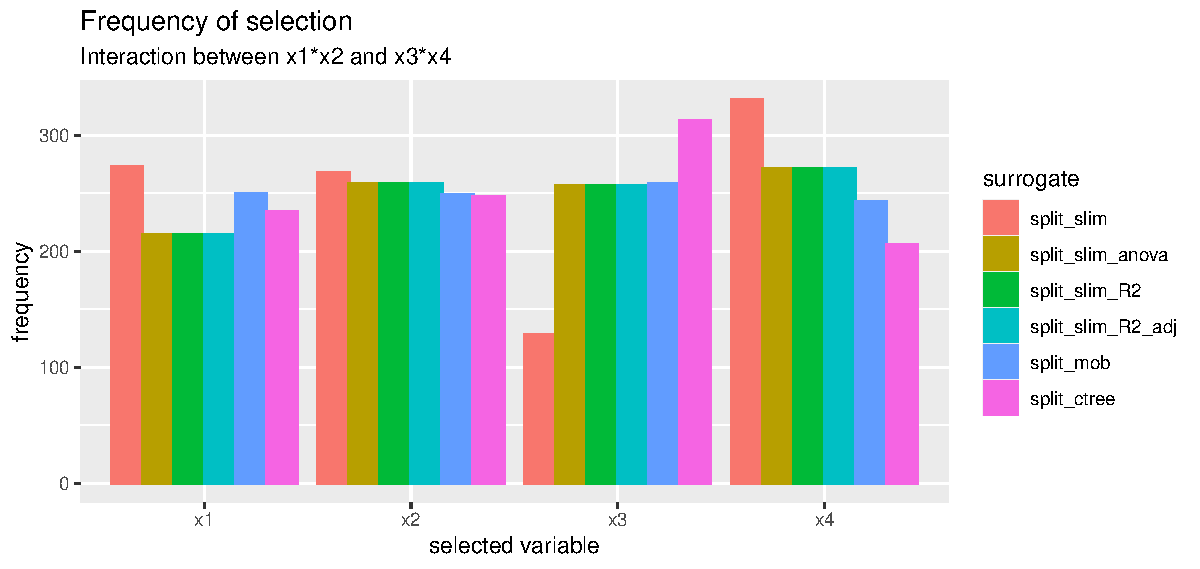
\includegraphics[width=11cm]{Figures/Selection_Bias/interaction_frequency.pdf}
\end{figure}

\end{frame}

\begin{frame}{Scenario Interaction full}

All $X_j \sim U(0,1)$; $X_3$ rounded to one digit, $X_4$ rounded to two digits\\
$Y = X_1 + X_2 + X_3 + X_4 + X_1 X_2 + X_1 X_3 + X_1 X_4 + X_2 X_3 + X_2 X_4 + X_3 X_4 + eps$
\begin{figure}
    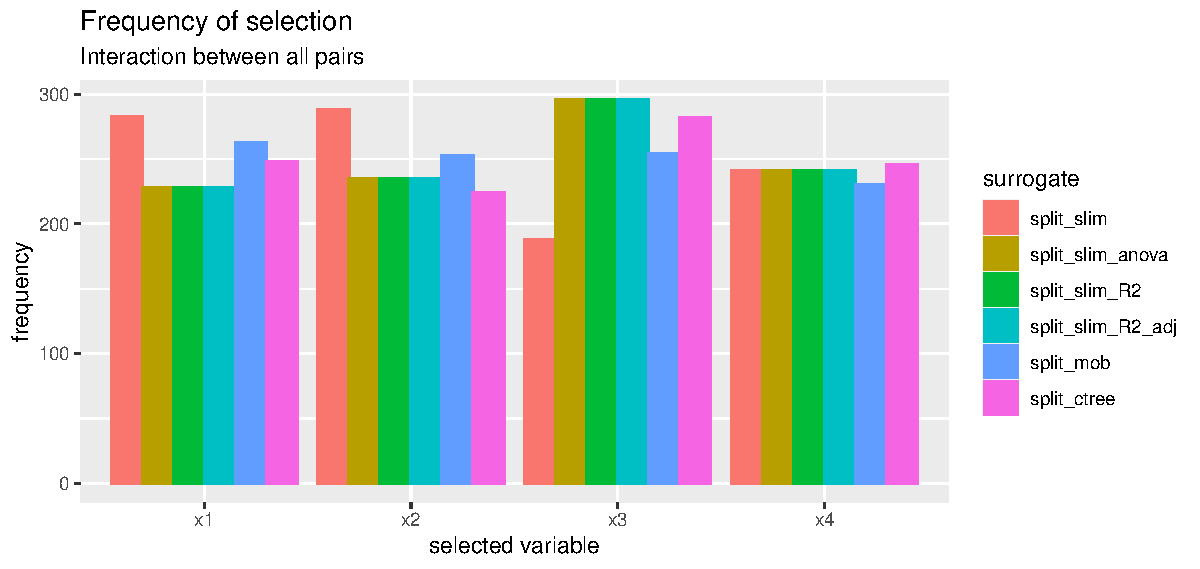
\includegraphics[width=11cm]{Figures/Selection_Bias/interaction_full_frequency.pdf}
\end{figure}

\end{frame}


\section{Performance}
\begin{frame}{Performance Comparison}
\textbf{Procedure:} 

For each simulation run (50 repetitions)
\begin{enumerate}
    \item create simulation data and perform train/test split (2/3)
    \item fit black box model (correct specified lm and xgboost model) to the training data and measure training and generalization performance ($R^2$ and MSE)
    \item For each model in SLIM, MOB, CTree fit surrogate model to the original training data to measure accuracy (training and generalization) and to the blackbox output to measure fidelity (training and generalization)
\end{enumerate}

\textbf{Note:} All three Methods are forced to generate models with the same terminal node size, i.e. no pruning except fixed tree depth and minimum node size is used
\end{frame}



\begin{frame}{Linear Smooth}
\textbf{Data} ($n= 1500$):
\begin{itemize}
    \item $X_1,..., X_5 \sim U(-1,1)$, $X_6, X_7 \sim N(0,1)$, $\epsilon \sim N(0, sd_{data})$
    \item $ Y = X_1 + 4   X_2 + 3   X_2   X_3 + 4  X_4  X_5 + X_5 + \epsilon $
\end{itemize}

\begin{figure}
    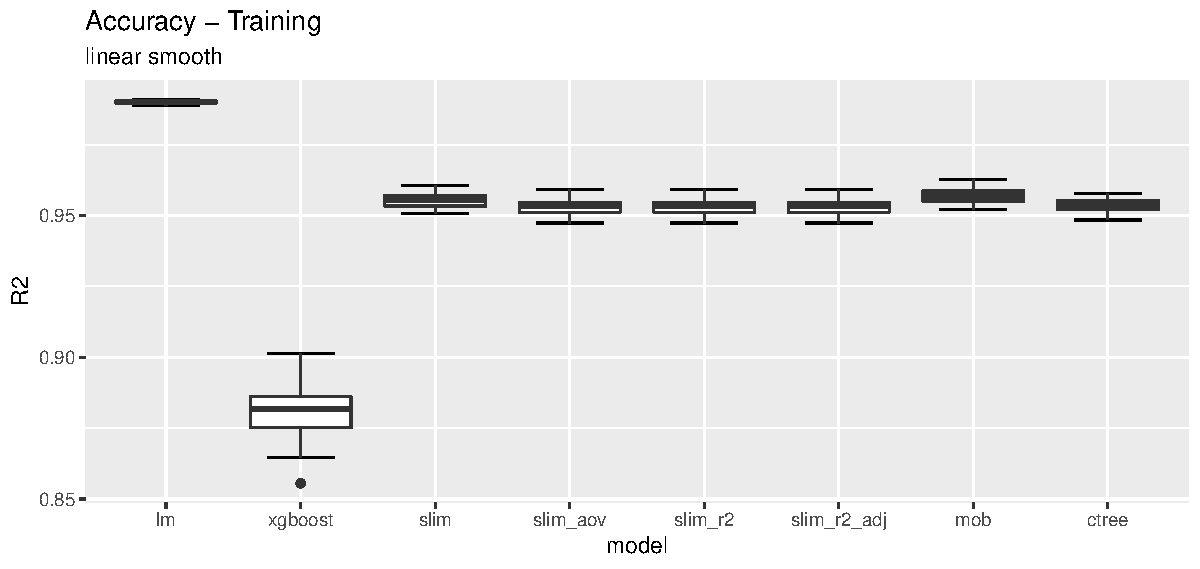
\includegraphics[width=11cm]{Figures/Performance/linear_smooth/r2_acc_train.pdf}
\end{figure}
\end{frame}

\begin{frame}{Linear Smooth - Fidelity}
\begin{figure}
    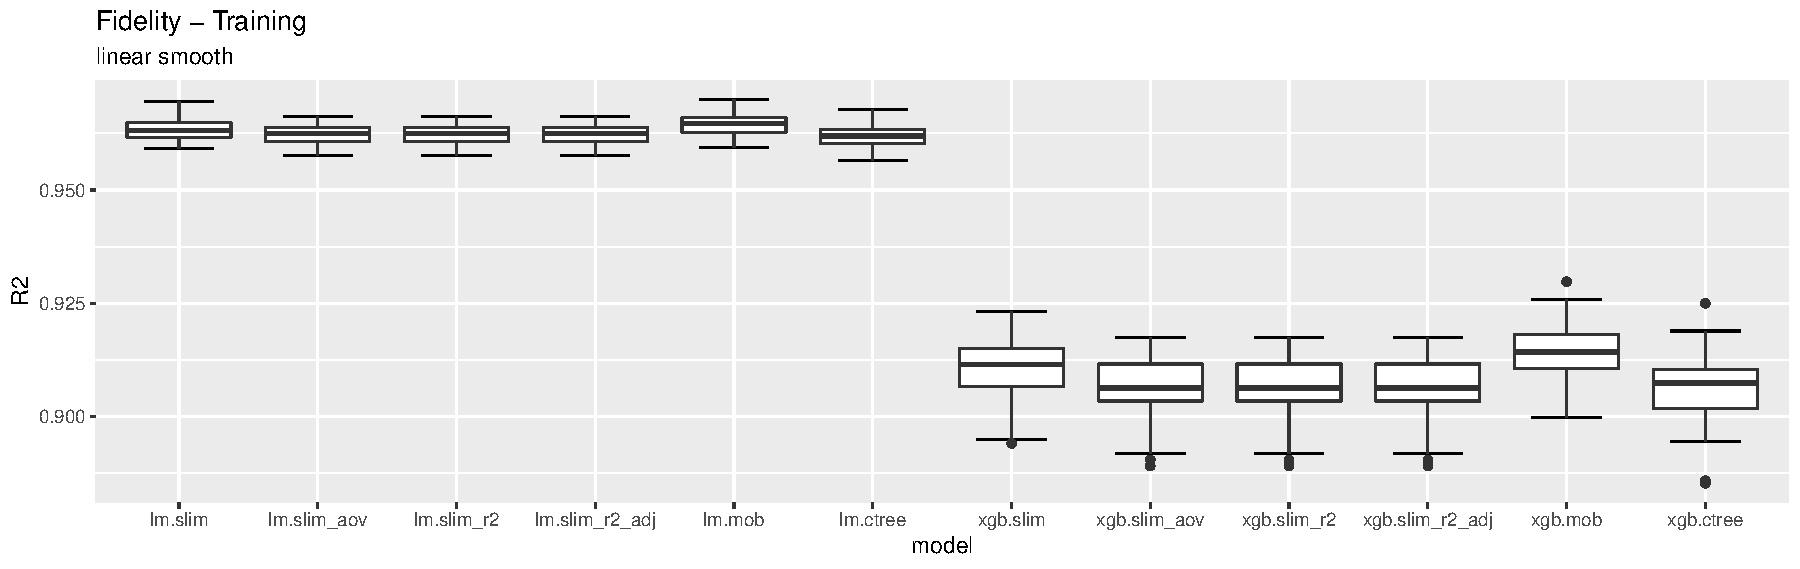
\includegraphics[width=11cm]{Figures/Performance/linear_smooth/r2_fidelity_train.pdf}
\end{figure}
    
\end{frame}

\begin{frame}{Linear Categorical}
\textbf{Data} ($n= 1500$):
\begin{itemize}
    \item $X_1, X_2 \sim U(-1,1)$, $X_3, ..., X_5 \sim Bern(0.5)$, $X_6 \sim N(0,1)$,  $\epsilon \sim N(0, sd_{data})$
    \item $ Y =  0.2  X_{1} - 8  X_2 + 16  X_2  \mathbf{I}_{X_3 = 0} + 8  X_2  \mathbf{I}_{X_1 > mean(X_1)} + \epsilon $
\end{itemize}

\begin{figure}
    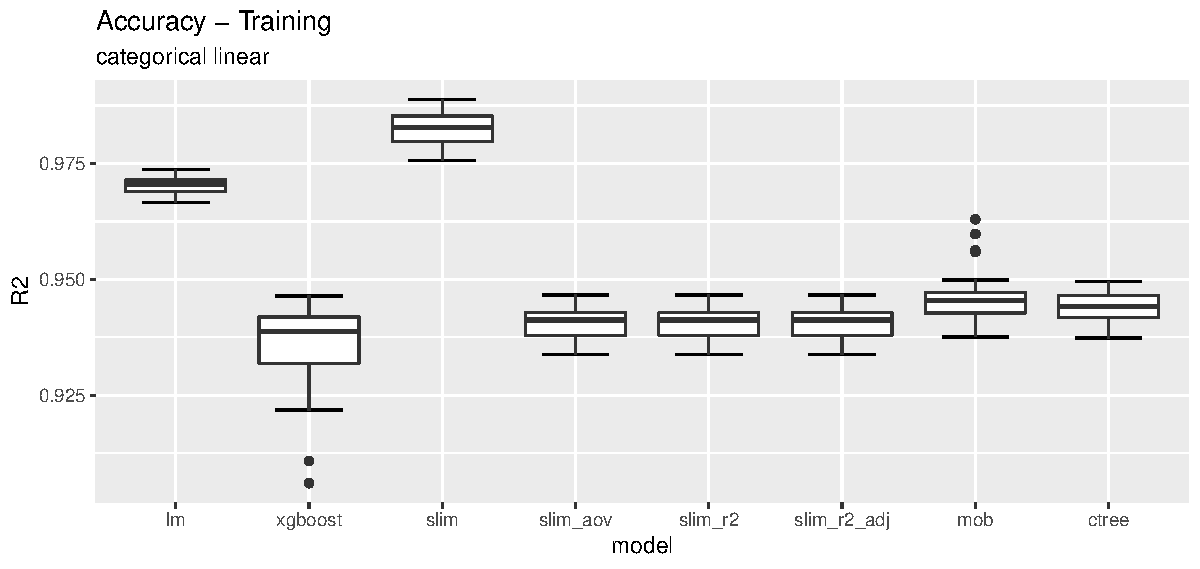
\includegraphics[width=11cm]{Figures/Performance/categorical_linear/r2_acc_train.pdf}
\end{figure}
\end{frame}

\begin{frame}{Linear Categorical - Fidelity}
\begin{figure}
    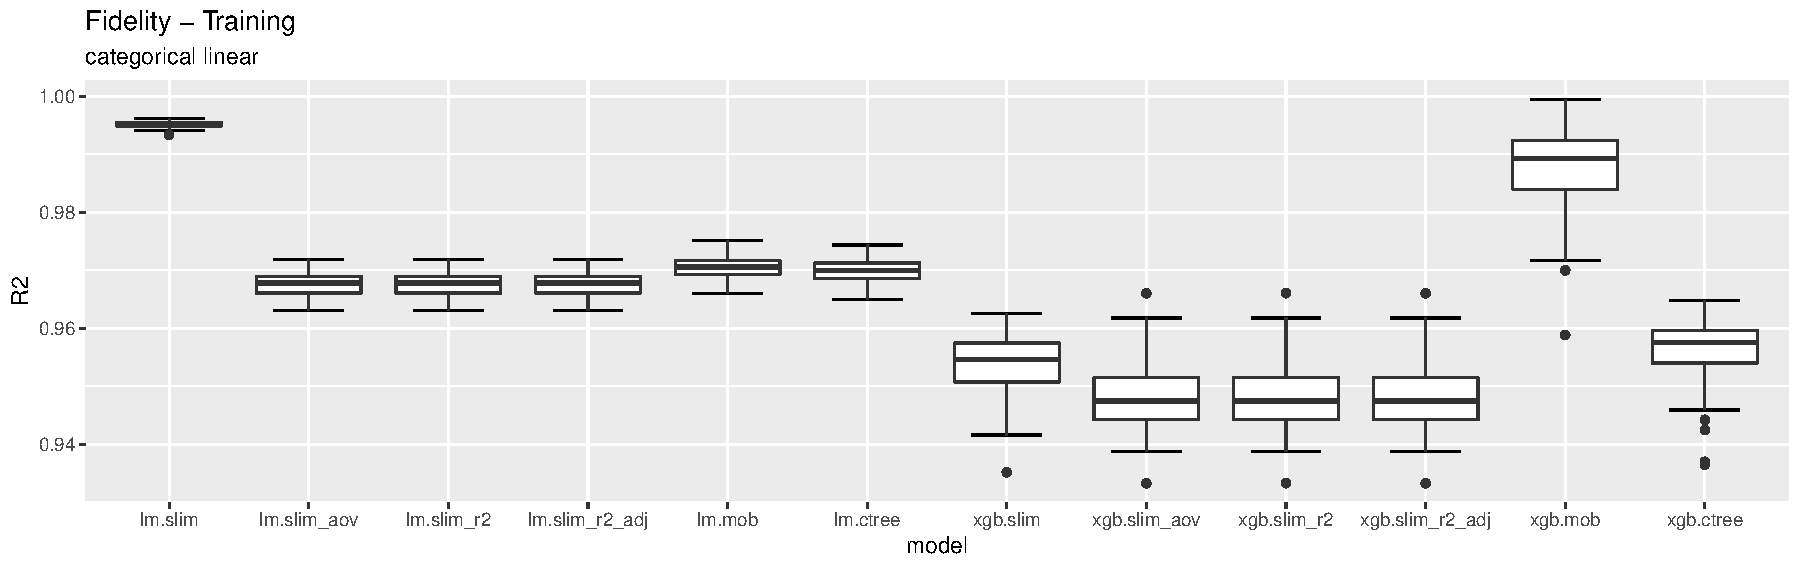
\includegraphics[width=11cm]{Figures/Performance/categorical_linear/r2_fidelity_train.pdf}
\end{figure}
\end{frame}

\begin{frame}{Linear Mixed}
\textbf{Data} ($n= 3000$):
\begin{itemize}
    \item $X_1, X_2 \sim U(-1,1)$, $X_3, ..., X_5 \sim Bern(0.5)$, $X_6, ... X_20 \sim N(0,1)$,  $\epsilon \sim N(0, sd_{data})$
    \item \begin{align*}
    Y = & 4   X_2 + 2   X_4 + 2   X_6 + 2   X_8 + 4   X_2   X_1 + 8   X_2   \mathbf{I}_{X_3 = 0} + 10   X_2   X_6    \mathbf{I}_{X_5 = 1} \\
    & + 8   X_2   X_7 + 3   X_1   X_3 + 3   X_8   X_{10} + 3   X_7   X_9     
    \end{align*}
    
\end{itemize}

\begin{figure}
    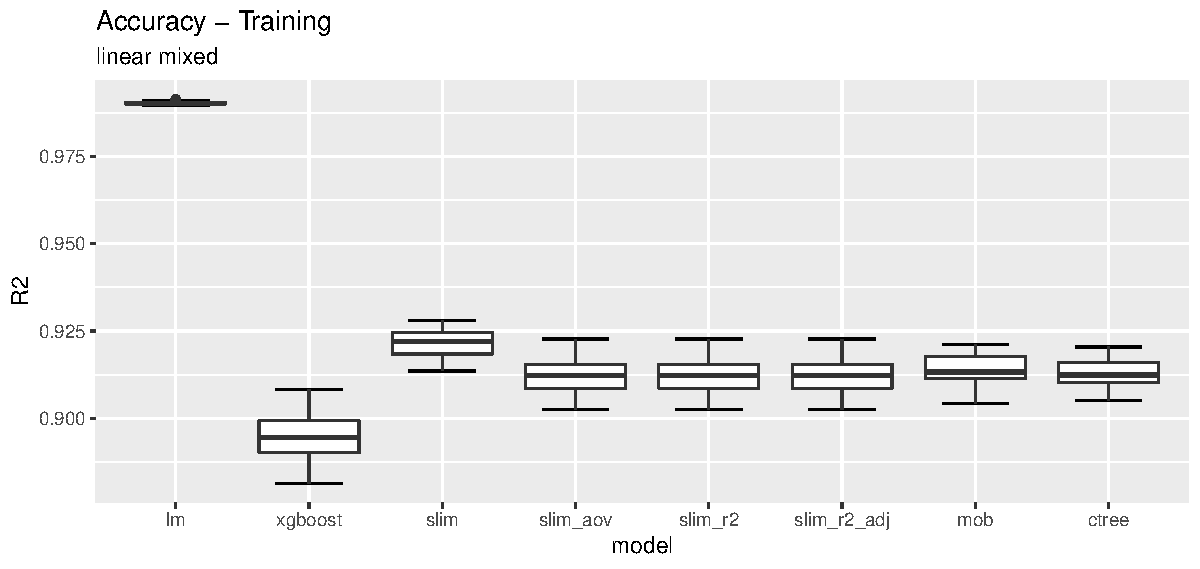
\includegraphics[width=11cm]{Figures/Performance/linear_mixed/r2_acc_train.pdf}
\end{figure}
\end{frame}

\begin{frame}{Linear Mixed - Fidelity}
\begin{figure}
    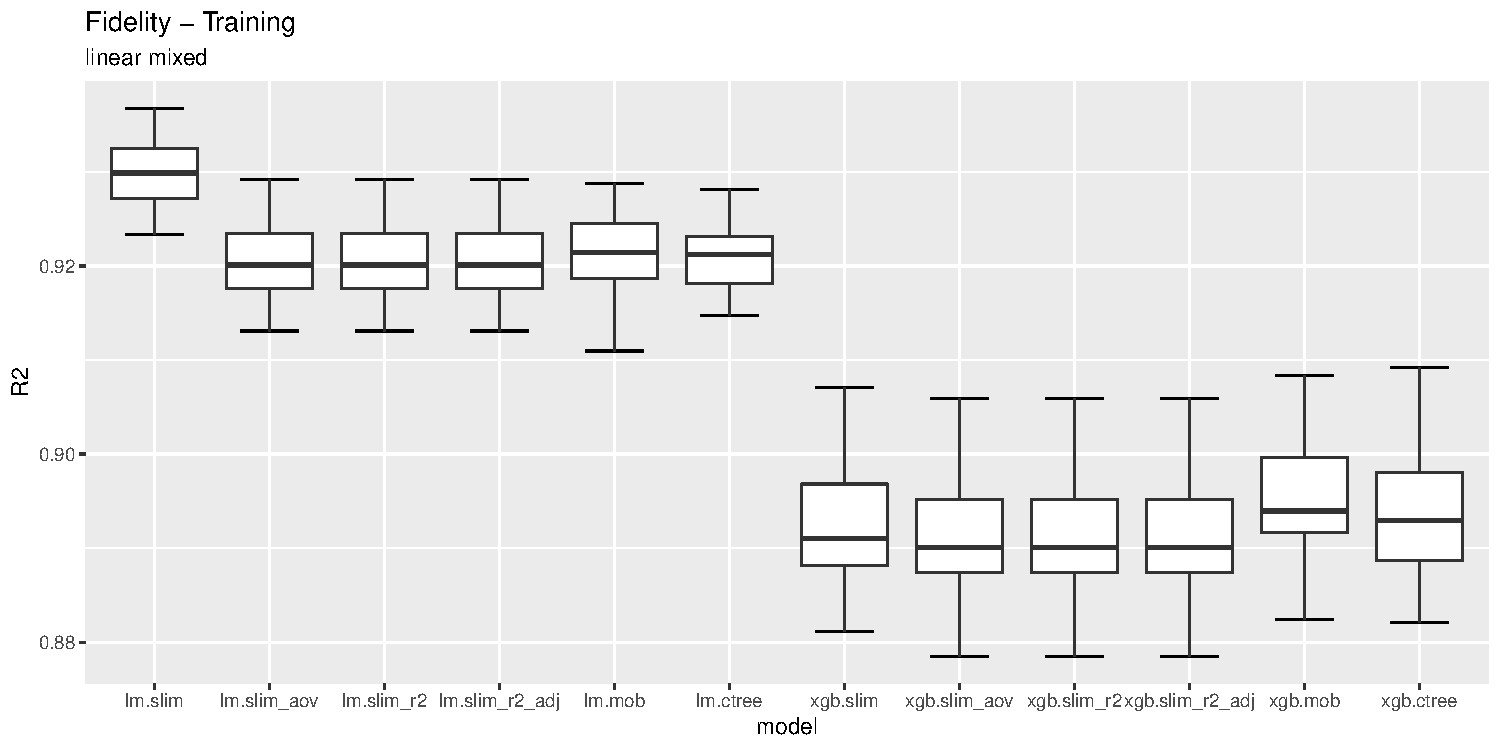
\includegraphics[width=11cm]{Figures/Performance/linear_mixed/r2_fidelity_train.pdf}
\end{figure}
\end{frame}


\section{Stability}
\begin{frame}{Stability Comparison}
\textbf{Procedure:} 
\begin{enumerate}
    \item create simulation data and train black box models on the data (this datasets are only used to train the black box model)
    \item for each simulation run 
    \begin{enumerate}
        \item create a new dataset and perform train/test split
        \item calculate blackbox predictions for the new dataset
        \item For each model in SLIM, MOB, CTree fit surrogate model to the new training dataset to measure accuracy (training and generalization) and to the new training data and the predicted blackbox output to measure fidelity (training and generalization)
        \item count number of terminal nodes in for the surrogate model and the tree based model on the original 
    \end{enumerate}
\end{enumerate}
\end{frame}

\begin{frame}{Linear Mixed}
\textbf{Data} ($n= 3000$):
\begin{itemize}
    \item $X_1, X_2 \sim U(-1,1)$, $X_3, ..., X_5 \sim Bern(0.5)$, $X_6, ... X_20 \sim N(0,1)$,  $\epsilon \sim N(0, sd_{data})$
    \item \begin{align*}
    Y = & 4   X_2 + 2   X_4 + 2   X_6 + 2   X_8 + 4   X_2   X_1 + 8   X_2   \mathbf{I}_{X_3 = 0} + 10   X_2   X_6    \mathbf{I}_{X_5 = 1} \\
    & + 8   X_2   X_7 + 3   X_1   X_3 + 3   X_8   X_{10} + 3   X_7   X_9     
    \end{align*}
    
\end{itemize}

\end{frame}

\begin{frame}{Linear Mixed}
\begin{figure}
    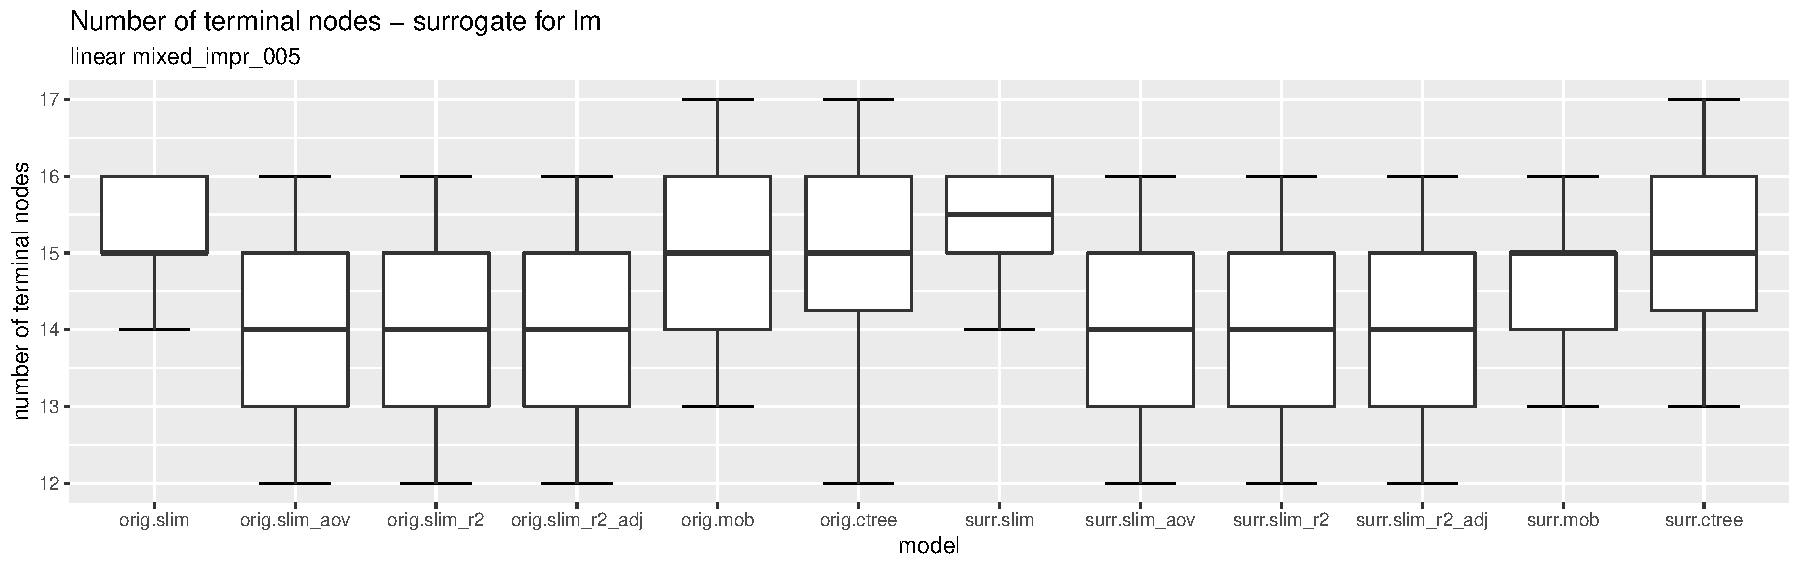
\includegraphics[width=11cm]{Figures/Stability/linear_mixed_impr_005/lm_nofnodes.pdf}
\end{figure}   

\begin{figure}
    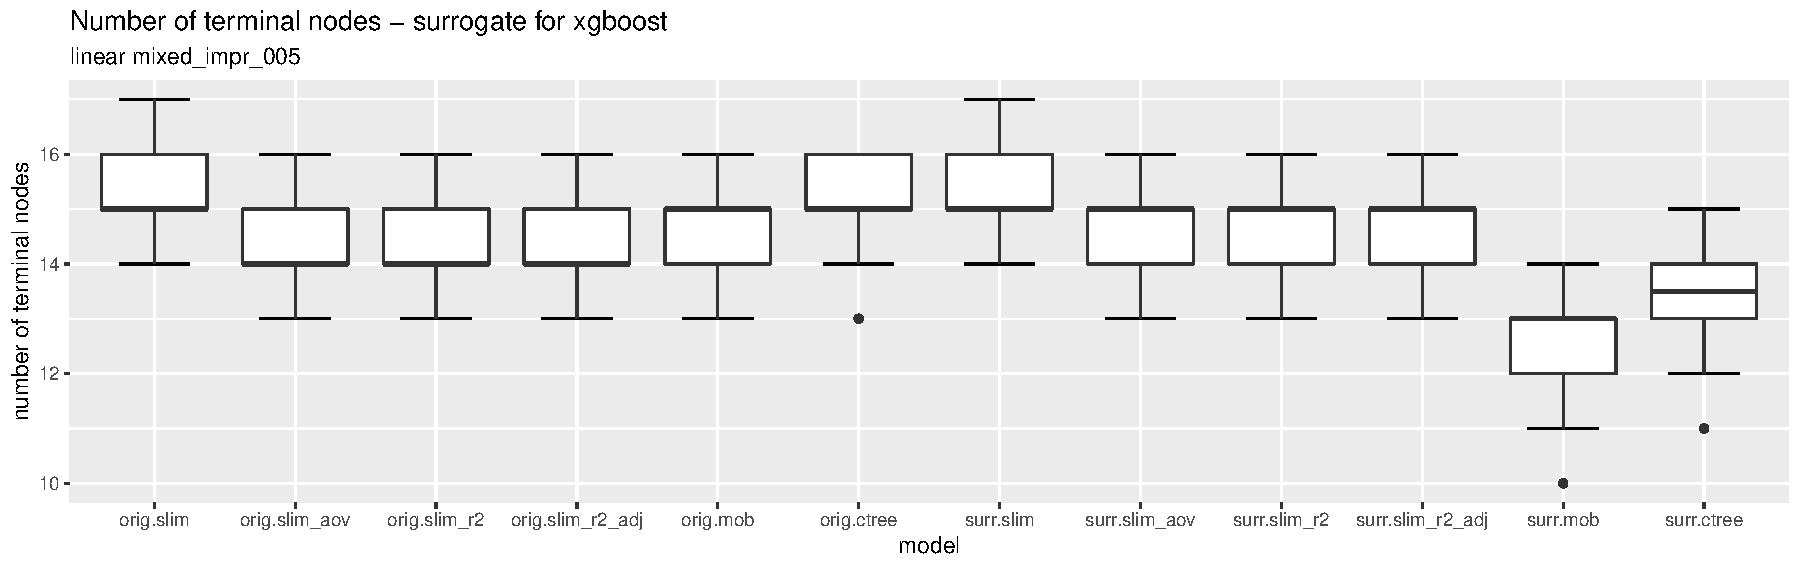
\includegraphics[width=11cm]{Figures/Stability/linear_mixed_impr_005/xgboost_nofnodes.pdf}
\end{figure}  

\end{frame}

\begin{frame}{Linear Mixed}
Selected split variables for depth 1 and 2 for Models based on \textbf{original data}\\
\textbf{SLIM}

\begin{table}[ht]
\centering
\begin{tabular}{lllrrr}
  \hline
depth & split\_id & feature & share & split.mean & split.sd \\ 
  \hline
1 & 0 & x2 & 1.00 & 0.01 & 0.05 \\ 
  2 & 0\_1 & x2 & 1.00 & -0.51 & 0.07 \\ 
  2 & 0\_2 & x2 & 0.92 & 0.51 & 0.07 \\ 
  2 & 0\_2 & x5 & 0.08 & 0.00 & 0.00 \\ 
   \hline
\end{tabular}
\end{table}

\textbf{MOB}
\begin{table}[ht]
\centering
\begin{tabular}{lllrrr}
  \hline
depth & split\_id & feature & share & split.mean & split.sd \\ 
  \hline
1 & 0 & x2 & 1.00 & 0.02 & 0.06 \\ 
  2 & 0\_1 & x2 & 0.58 & -0.49 & 0.06 \\ 
  2 & 0\_1 & x6 & 0.34 & 0.08 & 0.13 \\ 
  2 & 0\_1 & x5 & 0.08 & 0.00 & 0.00 \\ 
  2 & 0\_2 & x6 & 0.56 & -0.01 & 0.13 \\ 
  2 & 0\_2 & x2 & 0.44 & 0.50 & 0.05 \\ 
   \hline
\end{tabular}
\end{table}

\end{frame}


\begin{frame}{Linear Mixed}
Selected split variables for depth 1 and 2 for Models based on \textbf{lm predictions}\\
\textbf{SLIM}

\begin{table}[ht]
\centering
\begin{tabular}{lllrrr}
  \hline
depth & split\_id & feature & share & split.mean & split.sd \\ 
  \hline
1 & 0 & x2 & 1.00 & 0.02 & 0.05 \\ 
  2 & 0\_1 & x2 & 1.00 & -0.50 & 0.07 \\ 
  2 & 0\_2 & x2 & 0.94 & 0.52 & 0.07 \\ 
  2 & 0\_2 & x5 & 0.06 & 0.00 & 0.00 \\ 
   \hline
\end{tabular}
\end{table}

\textbf{MOB}
\begin{table}[ht]
\centering
\begin{tabular}{lllrrr}
  \hline
depth & split\_id & feature & share & split.mean & split.sd \\ 
  \hline
1 & 0 & x2 & 1.00 & 0.01 & 0.06 \\ 
  2 & 0\_1 & x2 & 0.60 & -0.48 & 0.06 \\ 
  2 & 0\_1 & x6 & 0.36 & 0.04 & 0.18 \\ 
  2 & 0\_1 & x5 & 0.04 & 0.00 & 0.00 \\ 
  2 & 0\_2 & x6 & 0.52 & -0.04 & 0.14 \\ 
  2 & 0\_2 & x2 & 0.46 & 0.50 & 0.05 \\ 
  2 & 0\_2 & x5 & 0.02 & 0.00 &  \\ 
   \hline
\end{tabular}
\end{table}
\end{frame}

\begin{frame}{Linear Mixed}
Selected split variables for depth 1 and 2 for Models based on \textbf{xgboost predictions}\\
\textbf{SLIM}

\begin{table}[ht]
\centering
\begin{tabular}{lllrrr}
  \hline
depth & split\_id & feature & share & split.mean & split.sd \\ 
  \hline
1 & 0 & x2 & 1.00 & -0.01 & 0.03 \\ 
  2 & 0\_1 & x2 & 1.00 & -0.50 & 0.07 \\ 
  2 & 0\_2 & x2 & 1.00 & 0.51 & 0.03 \\ 
   \hline
\end{tabular}
\end{table}

\textbf{MOB}
\begin{table}[ht]
\centering
\begin{tabular}{lllrrr}
  \hline
depth & split\_id & feature & share & split.mean & split.sd \\ 
  \hline
1 & 0 & x2 & 1.00 & -0.01 & 0.01 \\ 
  2 & 0\_1 & x2 & 1.00 & -0.53 & 0.05 \\ 
  2 & 0\_2 & x2 & 1.00 & 0.51 & 0.01 \\ 
   \hline
\end{tabular}
\end{table}
\end{frame}


\begin{frame}{Bibliography}
    \bibliography{bibliography}
    \bibliographystyle{dcu}

\end{frame}
\end{document}